% =========================================================
%  ¿Crisis de seguridad o cambio cualitativo?
%  Evidencia sobre delitos violentos contra la propiedad
%  en Chile, 2013--2025
%  Compilar: pdflatex → bibtex → pdflatex → pdflatex
% =========================================================
\documentclass[12pt,a4paper]{article}

\usepackage[utf8]{inputenc}
\usepackage[T1]{fontenc}
\usepackage{geometry}
\geometry{left=3cm,right=2.5cm,top=3cm,bottom=3cm}
\linespread{1.5}
\usepackage{graphicx}
\usepackage{booktabs}
\usepackage{amsmath}
\usepackage{amssymb}
\usepackage{array}
\usepackage{longtable}
\usepackage{float}
\usepackage{caption}
\usepackage{xcolor}
\usepackage[expansion=false]{microtype}
\usepackage{natbib}
\usepackage{fancyhdr}
\usepackage{parskip}
\usepackage{hyperref}
\hypersetup{
  colorlinks=true,
  linkcolor=black,
  citecolor=black,
  urlcolor=blue
}

\graphicspath{{../output/figures/}}

\pagestyle{fancy}
\fancyhf{}
\rhead{\footnotesize Delitos violentos contra la propiedad en Chile, 2013--2025}
\lhead{\footnotesize \thepage}
\renewcommand{\headrulewidth}{0.4pt}

\newcommand{\tablenote}[1]{%
  \vspace{2pt}%
  \begin{minipage}{\linewidth}%
    \footnotesize\textit{Nota:} #1%
  \end{minipage}%
}

\setcitestyle{authoryear,round,semicolon}

% =========================================================
\begin{document}
% =========================================================

\thispagestyle{plain}

\begin{center}
{\Large\bfseries \textquestiondown Crisis de seguridad o cambio cualitativo?\\[6pt]
Evidencia sobre los delitos violentos contra la propiedad\\[6pt]
en Chile, 2013--2025}

\vspace{18pt}
{\normalsize Ariel Valdebenito\textsuperscript{a} \quad Crist\'obal Cares\textsuperscript{b}}

\vspace{6pt}
{\small \textsuperscript{a}Instituto Nacional de Estad\'isticas, Santiago, Chile \quad
\textsuperscript{b}Universidad de Santiago de Chile}

\vspace{6pt}
{\small Marzo de 2026}
\end{center}

\vspace{12pt}
\noindent\rule{\linewidth}{0.5pt}
\vspace{4pt}

\begin{quote}
\small\noindent\textbf{Resumen.} Este art\'iculo examina si el aumento percibido en la violencia
patrimonial en Chile refleja un incremento real y estructural en el volumen de delitos,
o un cambio cualitativo en la composici\'on de los mismos. Utilizando un panel de
denuncias registradas por Carabineros de Chile para 16 regiones y 156 meses (2013--2025),
estimamos modelos Poisson-QMLE con spline c\'ubico restringido e inferencia por Wild
Cluster Bootstrap, complementados con tests CUSUM-GLM regional y detecci\'on de
quiebres de Bai-Perron. Los resultados muestran que los dos tipos de robo con violencia
dominantes concentran el 93\% del grupo. La tasa agregada de robos violentos aument\'o
respecto al Spline~1 (2013--2016) y alcanz\'o un m\'aximo hist\'orico en 2023
(377 por 100.000 hab.), impulsada en parte por la emergencia del robo de veh\'iculo
con violencia o intimidaci\'on a partir de 2020, y describe una inflexi\'on descendente
en el Spline~4 m\'as reciente (2022--2025: IRR\,=\,0.868, $p=0.057$). Pese a ello, el ratio robos violentos/total patrimonial
alcanz\'o un m\'aximo hist\'orico de 21.6\% en enero de 2024, impulsado por la ca\'ida
m\'as pronunciada de los robos no violentos. El debate sobre la ``crisis de seguridad''
captura algo real---la victimizaci\'on directa es m\'as probable incluso cuando el
n\'umero total de robos baja---pero sobreestima el fen\'omeno al confundir volumen con
composici\'on.

\vspace{6pt}
\noindent\textbf{Palabras clave:} Delitos contra la propiedad; robos violentos; cambio
estructural; Poisson-QMLE; panel regional; Chile.

\noindent\textbf{JEL:} K42; C23; R10.
\end{quote}

\vspace{4pt}
\noindent\rule{\linewidth}{0.5pt}

\bigskip

% =========================================================
\section{Introducci\'on}
% =========================================================

Chile ha vivido un debate sostenido sobre la percepci\'on de inseguridad ciudadana.
Desde el estallido social de octubre de 2019 y, con mayor intensidad, desde la
reactivaci\'on post-pandemia de 2022, la ``crisis de seguridad'' ha ocupado un lugar
central en la agenda p\'ublica, medi\'atica y legislativa. La delincuencia figura
sistem\'aticamente entre las principales preocupaciones de la ciudadan\'ia, y el debate
pol\'itico ha gravitado hacia propuestas de endurecimiento de penas y ampliaci\'on de
facultades policiales.

Sin embargo, el diagn\'ostico sobre la magnitud y naturaleza del fen\'omeno dista de
ser homog\'eneo. Los registros administrativos de Carabineros de
Chile---que para nuestros prop\'ositos anal\'iticos se limitan exclusivamente a las denuncias ciudadanas para aislar la demanda de seguridad---permiten distinguir
entre el \emph{volumen} total de delitos y la \emph{composici\'on} de ese volumen. Esta
distinci\'on es anal\'iticamente crucial: una sociedad puede experimentar una percepci\'on
creciente de inseguridad sin que el n\'umero absoluto de delitos violentos aumente, si
la proporci\'on de eventos de contacto directo con la v\'ictima crece respecto del total.
Esos eventos son los m\'as memorables y traum\'aticos, y determinan en mayor medida la
experiencia subjetiva de inseguridad.

La evidencia internacional sugiere que este tipo de cambio cualitativo es posible.
\citet{cohen1979} mostraron que la actividad rutinaria de v\'ictimas y victimarios
determina las oportunidades del delito: cuando esas oportunidades se contraen para
delitos de baja confrontaci\'on, pueden persistir---e incluso aumentar en participaci\'on
relativa---los delitos que dependen menos de la oportunidad y m\'as de la coerci\'on
directa. \citet{blumstein1988} documentaron un patr\'on similar en per\'iodos de
descenso generalizado de la criminalidad: los delitos que persisten tienden a ser los
de mayor lesividad.

Este art\'iculo eval\'ua emp\'iricamente si Chile experimenta una din\'amica de este
tipo. La pregunta central es: \textit{\textquestiondown Han aumentado estructuralmente
los delitos violentos contra la propiedad en Chile durante el per\'iodo 2013--2025,
o el incremento percibido refleja un cambio cualitativo en la composici\'on del delito
que no necesariamente implica m\'as v\'ictimas en t\'erminos absolutos?}

Nuestra contribuci\'on es triple. Primero, construimos un panel regional de casos
policiales para 16 regiones y 156 meses---la serie temporal m\'as larga analizada
sistem\'aticamente para este fen\'omeno en Chile---con correcci\'on demogr\'afica que
incorpora los flujos migratorios post-Censo 2017 a trav\'es de datos del Servicio
Nacional de Migraciones (SERMIG). Segundo, proponemos una clasificaci\'on tricot\'omica
que distingue robos violentos, robos por sorpresa y robos no violentos, capturando
din\'amicas cualitativamente distintas que quedan enmascaradas en las clasificaciones
binarias institucionales. Tercero, aplicamos estimaci\'on Poisson-QMLE con spline c\'ubico restringido e inferencia por Wild Cluster Bootstrap, complementada con detecci\'on de quiebres de Bai-Perron sobre el ratio nacional desestacionalizado; la estabilidad de los resultados se verifica con modelos de sensibilidad de clasificaci\'on reportados en el Ap\'endice.

El hallazgo central es parad\'ojico: el ratio robos violentos/total alcanz\'o su
m\'aximo hist\'orico (21.6\% en enero de 2024), pero esto no refleja un aumento en
el volumen de robos violentos, sino el declive m\'as pronunciado de los robos no
violentos, que reduce el denominador. Los dos tipos de robo que concentran el 93\% del grupo ---el robo con intimidaci\'on y el robo con violencia--- aumentaron respecto al Spline~1 (2013--2016) y describen un ciclo de ascenso hasta 2023 e inflexi\'on descendente en el Spline~4 (2022--2025). La ``crisis'' existe, pero su naturaleza es cualitativa, no cuantitativa.

El art\'iculo se organiza como sigue. La Secci\'on~\ref{sec:marco} presenta el marco
conceptual. La Secci\'on~\ref{sec:datos} describe los datos y la estrategia
metodol\'ogica. La Secci\'on~\ref{sec:resultados} expone los resultados en tres capas:
descriptiva, inferencial y de falsificaci\'on. La Secci\'on~\ref{sec:robustez} reporta
los an\'alisis de robustez. La Secci\'on~\ref{sec:discusion} discute las implicancias
y limitaciones. La Secci\'on~\ref{sec:conclusiones} concluye.


% =========================================================
\section{Marco conceptual}
\label{sec:marco}
% =========================================================

Los registros policiales de denuncias miden \emph{criminalidad aparente}: la fracci\'on de
delitos que llega a conocimiento de las autoridades. La diferencia entre criminalidad
real y aparente---la cifra negra del delito---depende de factores como la gravedad del hecho, la
confianza institucional y el costo de la denuncia. Esta \'ultima dimensi\'on es
especialmente relevante para Chile: la plataforma Comisaria Virtual de Carabineros ha
facilitado la denuncia digital desde aproximadamente 2016, con adopci\'on masiva
post-COVID. La digitalizaci\'on tiene efectos asim\'etricos sobre la cifra negra. Para
delitos de alta lesividad---robo con violencia, intimidaci\'on, retenci\'on de
v\'ictimas---la gravedad motiva el reporte independientemente del canal disponible.
Para delitos de baja lesividad---hurtos, robos sin confrontaci\'on directa---la
reducci\'on del costo de denuncia puede generar un incremento en los registros que no
refleja mayor victimizaci\'on real. Este sesgo opera de manera diferencial por
categor\'ia, lo que hace importante distinguir tipos de robo al analizar tendencias.

La distinci\'on entre volumen y composici\'on de la delincuencia patrimonial es el
punto de partida anal\'itico. El volumen mide el n\'umero total de hechos por unidad
de poblaci\'on; la composici\'on mide la proporci\'on de cada tipo en el total. Estas
dos dimensiones pueden moverse en direcciones opuestas: si los robos sin confrontaci\'on
directa caen m\'as r\'apido que los robos con confrontaci\'on, el ratio de violentos
sobre el total sube a\'un cuando el volumen absoluto de violentos tambi\'en baje. Este
mecanismo tiene una l\'ogica plausible desde la teor\'ia de las actividades rutinarias
\citep{cohen1979}: la expansi\'on del comercio electr\'onico, la mayor seguridad
residencial y los cambios en la movilidad cotidiana post-pandemia reducen las
oportunidades para el robo oportunista que depende de encuentros no planeados. Los
robos que requieren coerci\'on directa son menos sensibles a estas barreras
estructurales.

En el debate chileno, el an\'alisis se complejiza por la emergencia de fen\'omenos
delictuales vinculados al crimen organizado: el portonazo (robo de veh\'iculo por
violencia o intimidaci\'on), el secuestro expr\'es (retenci\'on de v\'ictimas para
coerci\'on de transferencias bancarias) y la violencia letal territorial. Estos
fen\'omenos pueden aumentar en t\'erminos relativos---o incluso absolutos---aunque el
volumen agregado de la delincuencia patrimonial disminuya, y generan una experiencia
subjetiva de inseguridad elevada incluso cuando los \'indices globales muestran
descenso. Distinguir estas se\~nales emergentes del ruido estad\'istico del total, y
separar cambios de composici\'on de cambios de volumen, es la contribuci\'on
metodol\'ogica central de este trabajo.


% =========================================================
\section{Datos y metodolog\'ia}
\label{sec:datos}
% =========================================================

\subsection{Fuentes de datos y muestra}

La fuente principal es el sistema de registros administrativos de Carabineros de Chile
(CCH), publicados por el Instituto Nacional de Estad\'isticas en las Estad\'isticas de
Seguridad y Justicia \citep{INE2026}. El universo de an\'alisis es un panel elaborado
exclusivamente sobre la base de denuncias formales por delitos contra la propiedad
para las 16 regiones del pa\'is en el per\'iodo enero de 2013 a diciembre de 2025,
generando $N = 16 \times 156 = 2{,}496$ observaciones regi\'on-mes. Las denuncias fungen
como proxy de la criminalidad conocida por las polic\'ias (\textit{crimes known to
police} en la terminolog\'ia anglosajona): hechos que llegan a conocimiento de
Carabineros por denuncia directa de la v\'ictima o terceros. Es cr\'itico destacar que
se excluyen de la variable dependiente central las detenciones en flagrancia. Esta
decisi\'on asegura que el indicador mida de manera limpia la demanda ciudadana por
seguridad (victimizaci\'on aparente) y no se contamine con shocks en la oferta
institucional (proactividad u operativos policiales focalizados). La diferencia entre este
registro y la criminalidad real---la cifra negra---depende de la propensi\'on a denunciar,
el reconocimiento del hecho como delito y la confianza institucional.

Como fuente de triangulaci\'on con subreporte insignificante o cifra negra residual m\'inima
se utiliza el Registro de Homicidios Confirmados del Centro de Prevenci\'on de
Homicidios Violentos (CPHDV), con conteos anuales validados interinstitucionalmente para el per\'iodo
2018--2025. Su car\'acter de registro exhaustivo lo hace id\'oneo como validaci\'on
externa de las tendencias inferidas desde los datos CCH.

Las tasas de delincuencia se calculan con dos fuentes del Instituto Nacional de
Estad\'isticas. Para el panel regional---base del an\'alisis inferencial---se emplean
las proyecciones con Base Censo 2017 desagregadas por regi\'on. Para las estad\'isticas
descriptivas nacionales se utilizan las proyecciones con Base Censo 2024,
metodol\'ogicamente superiores por incorporar evidencia censal m\'as
reciente.\footnote{Las proyecciones INE con Base Censo 2024 est\'an disponibles
\'unicamente a nivel nacional al momento de este an\'alisis. La desagregaci\'on
regional a\'un no ha sido publicada, por lo que el panel de modelamiento mantiene la
Base 2017.} Sobre las proyecciones INE Base 2017 se aplica una correcci\'on migratoria
acumulativa sumando los flujos de residencias temporales y definitivas otorgadas por
SERMIG desde 2018.

\subsection{Clasificaci\'on tricot\'omica}
\label{sub:clasificacion}

La Codificaci\'on Nacional Penal (CNP) ordena el cat\'alogo de delitos
mediante C\'odigos \'Unicos de Materia (CUM). Entre \'estos, los delitos
contra la propiedad quedan organizados en dos grandes bloques:
\textit{Robos} ---que incluye tanto los robos con confrontaci\'on directa
o intimidaci\'on como el robo por sorpresa--- y \textit{Robos no violentos}.

La \textit{International Classification of Crime for Statistical Purposes}
(ICCS) de la UNODC propone, en cambio, un criterio diferente: sit\'ua el
robo por sorpresa o carterismo bajo la secci\'on~05 (\textit{Actos contra
la propiedad solamente}), y no en la secci\'on~04 (\textit{Actos contra la
propiedad que entra\~nan violencia o amenaza de violencia contra las
personas}). El fundamento es que el arrebatamiento sin confrontaci\'on
armada ---aunque pueda implicar contacto f\'isico moment\'aneo--- no
entra\~na la misma dimensi\'on de violencia interpersonal que el robo con
intimidaci\'on de arma o con resultado lesivo. En ese sentido, la diferencia
entre la CNP y la ICCS no es de jerarqu\'ia sino de criterio: ambas reflejan
formas distintas ---y en parte complementarias--- de clasificar la violencia
patrimonial.

Desde el punto de vista anal\'itico, esta distinci\'on importa. El robo
por sorpresa y los robos con confrontaci\'on directa presentan din\'amicas
cualitativamente distintas ante shocks externos: el estallido social de 2019
elev\'o con mayor intensidad los robos con confrontaci\'on directa, mientras
que la pandemia colaps\'o de forma m\'as pronunciada los arrebatos en el
espacio p\'ublico ---fuertemente dependientes de la aglomeraci\'on de
transeuntes y del transporte colectivo. Al agrupar ambas modalidades bajo
una misma categor\'ia, como hace la CNP, se enmascara esa heterogeneidad.
Proponemos, en consecuencia, una \textbf{clasificaci\'on tricot\'omica} (C3)
que introduce el robo por sorpresa como categor\'ia independiente. Sus tres
componentes ---detallados en la Tabla~\ref{tab:c3}--- son:

\begin{itemize}
  \item \textbf{Robos violentos:} fuerza directa sobre las personas,
    intimidaci\'on grave o resultado lesivo.\footnote{Incluye los tipos
    conocidos popularmente como ``encerronas'' y ``portonazos'' (robo de
    veh\'iculo con violencia o intimidaci\'on), as\'i como los robos con
    resultado de homicidio, violaci\'on o lesiones graves.}
  \item \textbf{Robos por sorpresa:} arrebatamiento en el espacio p\'ublico
    sin confrontaci\'on armada.\footnote{Denominado popularmente
    ``lanzazo'' o, en su versi\'on motorizada, ``motochorros''.}
  \item \textbf{Robos no violentos:} sustracci\'on sin confrontaci\'on
    directa con la v\'ictima.
\end{itemize}

Las alternativas dicot\'omicas ---clasificaci\'on institucional C1, que
mantiene el robo por sorpresa dentro del bloque de robos violentos, y la
variante ajustada C2--- se eval\'uan formalmente en el Ap\'endice~\ref{ap:clasif}.
Su comparaci\'on con C3 muestra que fusionar el robo por sorpresa con los
robos violentos oscurece las diferencias de respuesta ante shocks de
movilidad, lo que valida la separaci\'on tricot\'omica como la
parametrizaci\'on m\'as informativa disponible con datos administrativos
chilenos.

\begin{table}[H]
\centering
\caption{Clasificaci\'on tricot\'omica C3: c\'odigos \'unicos de materia (CUM) incluidos}
\label{tab:c3}
\small
\begin{tabular}{p{3.5cm}rp{7cm}}
\toprule
\textbf{Categor\'ia} & \textbf{CUM} & \textbf{Glosa} \\
\midrule
\multicolumn{3}{l}{\textit{C3.1 --- Robos violentos}} \\
 & 802 & Robo con intimidaci\'on \\
 & 803 & Robo con violencia \\
 & 827 & Robo con homicidio \\
 & 828 & Robo con violaci\'on \\
 & 829 & Robo con castraci\'on, mutilaci\'on o lesiones graves \\
 & 861 & Robo con lesiones graves \\
 & 862 & Robo con retenci\'on de v\'ictimas \\
 & 867 & Robo de veh\'iculo por violencia/intimidaci\'on (portonazo)\textsuperscript{a} \\
\midrule
\multicolumn{3}{l}{\textit{C3.2 --- Robos por sorpresa}} \\
 & 804 & Robo por sorpresa (``lanzazo'') \\
\midrule
\midrule
\multicolumn{3}{l}{\textit{Robos no violentos}} \\
 & 808 & Robo en bienes nacionales de uso p\'ublico (incluye accesorios automotrices) \\
 & 809 & Robo en lugar habitado \\
 & 810 & Robo en lugar no habitado \\
 & 821, 826, 846--848, 853, 13028 & Hurtos simples y afines \\
 & 831, 868 & Robo de veh\'iculo sin violencia \\
 & 858 & Robo con fuerza de cajeros autom\'aticos \\
 & 870--872 & Robo/hurto en ocasi\'on de calamidad; saqueo \\
 & 891, 892 & Sustracci\'on de madera \\
\bottomrule
\end{tabular}
\tablenote{\textsuperscript{a} El CUM 867 aparece con volumen significativo en el
sistema desde 2020; su exclusi\'on se eval\'ua en la Secci\'on~\ref{sec:robustez}.
Excluidos de las agrupaciones principales: receptaci\'on (CUM 812, 864, 869, 2009, 12053).
Adicionalmente cabe destacar: 1 UTM equivale a 69.542 CLP a diciembre de 2025.}
\end{table}

\subsection{Correcci\'on demogr\'afica y denominadores}
\label{sub:pop}

Las proyecciones INE Base 2017 proveen estimaciones anuales de poblaci\'on por regi\'on.
Para obtener el offset mensual requerido por el modelo, se interpola linealmente entre
a\~nos contiguos:
\[
  \text{Pop}_{\text{mes}}(r,y,m)
  = \text{Pop}_{\text{corr}}(r,y)
  + \frac{m - 6.5}{12}
  \bigl[\text{Pop}_{\text{corr}}(r,y+1) - \text{Pop}_{\text{corr}}(r,y)\bigr],
\]
donde $m \in \{1,\ldots,12\}$ es el mes del a\~no. El denominador corregido incorpora
los flujos migratorios post-Censo 2017 mediante el acumulado de residencias definitivas
y temporales otorgadas por SERMIG desde 2018:
\[
  \text{Pop}_{\text{corr}}(r,t)
  = \text{Pop}_{\text{INE}}(r,t)
  + \sum_{y=2018}^{t}\bigl[\text{RD}_{\text{otorga}}(r,y) + \text{RT}_{\text{otorga}}(r,y)\bigr].
\]
Esta correcci\'on (donde RD corresponde a Residencias Definitivas y RT a Residencias Temporales)
es una cota inferior de la poblaci\'on real, pues solo captura
migrantes formalmente regularizados. La sensibilidad a supuestos sobre la poblaci\'on
irregular se eval\'ua en la Secci\'on~\ref{sec:robustez}.

\subsection{Estrategia econom\'etrica}

Sea $Y_{rm}$ el conteo mensual de casos policiales en la regi\'on $r$ en el mes $m$.
El modelo principal especifica:
\begin{equation}
  \ln(\mu_{rm})
  = \sum_{k=2}^{12} \alpha_k \mathbf{1}(\text{mes}=k)
  + \delta_1 D^{\text{est}}_m + \delta_2 D^{\text{pan}}_m
  + f(t) + \sum_{r=2}^{16} \lambda_r \mathbf{1}(\text{regi\'on}=r)
  + \ln(\text{Pop}_{\text{mes},rt}),
  \label{eq:poisson}
\end{equation}
donde $\sum \alpha_k$ captura la estacionalidad mensual (referencia: enero);
$D^{\text{est}}_m$ es una variable dicot\'omica para el estallido social (octubre de
2019 a febrero de 2020, 5 meses); $D^{\text{pan}}_m$ para la pandemia (marzo de 2020
a diciembre de 2021, 22 meses); $f(t)$ es un spline c\'ubico restringido con nodos
en los percentiles P25, P50 y P75 de la tendencia temporal; $\lambda_r$ son efectos
fijos regionales; y el offset $\ln(\text{Pop}_{\text{mes},rt})$ transforma el modelo
de conteos en uno de tasas. El t\'ermino $\ln(\text{Pop}_{\text{mes},rt})$ opera como \textit{offset}: fija su coeficiente en 1.0 y convierte el modelo de conteos en un modelo de tasas, de modo que los coeficientes reflejan cambios en la tasa de incidencia por 100.000 habitantes.

Los cuatro tramos del spline, con nodos en P25 (mes 39, $\approx$ marzo de 2016),
P50 (mes 78, $\approx$ junio de 2019) y P75 (mes 117, $\approx$ septiembre de 2022),
corresponden aproximadamente a: (i) enero de 2013--marzo de 2016; (ii) marzo de
2016--junio de 2019; (iii) junio de 2019--septiembre de 2022; y (iv) septiembre de
2022--diciembre de 2025. Esta parametrizaci\'on es agn\'ostica: los nodos se ubican
en percentiles del rango temporal sin imponer pre-supuestos sobre cu\'ando ocurre el
quiebre estructural, dejando que los datos determinen la forma funcional de la tendencia.

Se elige Poisson-QMLE frente a alternativas por tres razones. Frente a la regresi\'on
binomial negativa: el estimador QMLE es consistente aunque la varianza sea mal
especificada, y el Wild Cluster Bootstrap (WCB) neutraliza la sobredispersi\'on
residual sin imponer supuestos distribucionales adicionales. La estimaci\'on Poisson-QMLE (\textit{Quasi-Maximum Likelihood}) es consistente si la media condicional est\'a correctamente especificada ---incluso cuando la varianza no sigue la ley de Poisson--- gracias a que la funci\'on de puntuaci\'on del Poisson depende \'unicamente del primer momento. Formalmente, el estimador QMLE resuelve las ecuaciones de puntuaci\'on $\sum_{i}(y_i - \mu_i)\mathbf{x}_i = 0$, que son condiciones de primer orden v\'alidas bajo cualquier distribuci\'on de conteos con $E[Y|\mathbf{x}] = \exp(\mathbf{x}'\boldsymbol{\beta})$ \citep{gourieroux1984,wooldridge2010}. La sobredispersi\'on residual se aborda mediante el Wild Cluster Bootstrap. Frente al trend lineal
con nodos fijos: el spline con nodos agn\'osticos en percentiles no impone
pre-supuestos sobre cu\'ando ocurre el quiebre. Y frente a los errores est\'andar de
Huber-White: con $G=16$ clusters (regiones), estos son inconsistentes; el WCB con
pesos de Webb ($B=9{,}999$ replicaciones) provee inferencia v\'alida para este n\'umero
reducido de clusters \citep{cameron2015,mackinnon2023}. Se reportan Incidence Rate
Ratios ($\text{IRR} = e^\beta$), p-valores WCB e intervalos de confianza al 95\% por
inversi\'on.

El an\'alisis se complementa con tres procedimientos. El test CUSUM-GLM regional
ajusta un Poisson-GLM base por regi\'on, calcula el proceso emp\'irico de fluctuaci\'on
\citep{zeileis2002} y aplica el test supremo de puente browniano; los 16 p-valores se
ajustan por la tasa de descubrimientos falsos (FDR) de Benjamini-Hochberg. La
detecci\'on de quiebres de \citet{bai1998} se aplica al ratio mensual desestacionalizado
robos violentos/(violentos + no violentos) con errores HAC, seleccionando el n\'umero
\'optimo por BIC. Finalmente, un modelo de interacciones macrozona $\times$ spline
---donde macrozona agrupa regiones por proximidad geogr\'afica: Norte (Arica y Parinacota, Tarapac\'a, Antofagasta, Atacama y Coquimbo), Centro (Valpara\'iso, O'Higgins y Maule), Regi\'on Metropolitana, Sur (Biob\'io, La Araucan\'ia, Los R\'ios, \~Nuble y Los Lagos) y Austral (Ays\'en y Magallanes)---permite evaluar si la tendencia de largo plazo difiere entre zonas
geogr\'aficas; sus coeficientes se presentan en el Ap\'endice~\ref{ap:macro}.

La especificaci\'on se valida mediante dos modelos placebo. El placebo negativo (P1)
usa el cuasidelito vehicular, que deber\'ia crecer post-pandemia por el
retorno de la actividad vial. El placebo positivo (P2) usa los homicidios dolosos ---homicidio simple, homicidio calificado y homicidio en ri\~na, excluyendo cuasidelitos para aislar la violencia letal intencional--- cuya cifra negra es residual: los homicidios generan obligaci\'on institucional de investigaci\'on independientemente de que exista denuncia formal, y la convergencia entre los registros CCH y el CPHDV ---que valida cada caso mediante ficha m\'edica o autopsia--- da cuenta de una tasa de reporte cercana al 100\%. Si la violencia real est\'a aumentando, los homicidios deben mostrar tendencia convergente. Un modelo
adicional sobre los homicidios confirmados del CPHDV (2018--2025) provee triangulaci\'on
externa.


% =========================================================
\section{Resultados}
\label{sec:resultados}
% =========================================================

\subsection{Composici\'on y tendencias descriptivas}
\label{sub:descriptivo}

Entre enero de 2013 y diciembre de 2025, la serie mensual de casos policiales por
categor\'ia C3 articula tres episodios que son clave para entender la din\'amica de
la criminalidad patrimonial en Chile. Durante el estallido social (octubre de 2019 a
febrero de 2020), los robos violentos y los robos por sorpresa experimentaron alzas
transitorias mientras que los robos no violentos permanecieron pr\'acticamente
inalterados---una asimetr\'ia que sugiere que el desorden social activ\'o el delito
de confrontaci\'on directa pero no alter\'o la din\'amica de oportunidad de los robos
sin contacto con v\'ictimas. Vino despu\'es un colapso generalizado durante la
pandemia, m\'as pronunciado para los robos por sorpresa---que dependen de la
circulaci\'on de personas en el espacio p\'ublico---que para los robos violentos. En
la reactivaci\'on post-pandemia (2022--2025) los tres tipos se recuperaron sin retomar
los niveles del quinquenio previo, medidos en tasas por 100.000 habitantes
(Figura~\ref{fig:serie}).

\begin{figure}[H]
\centering
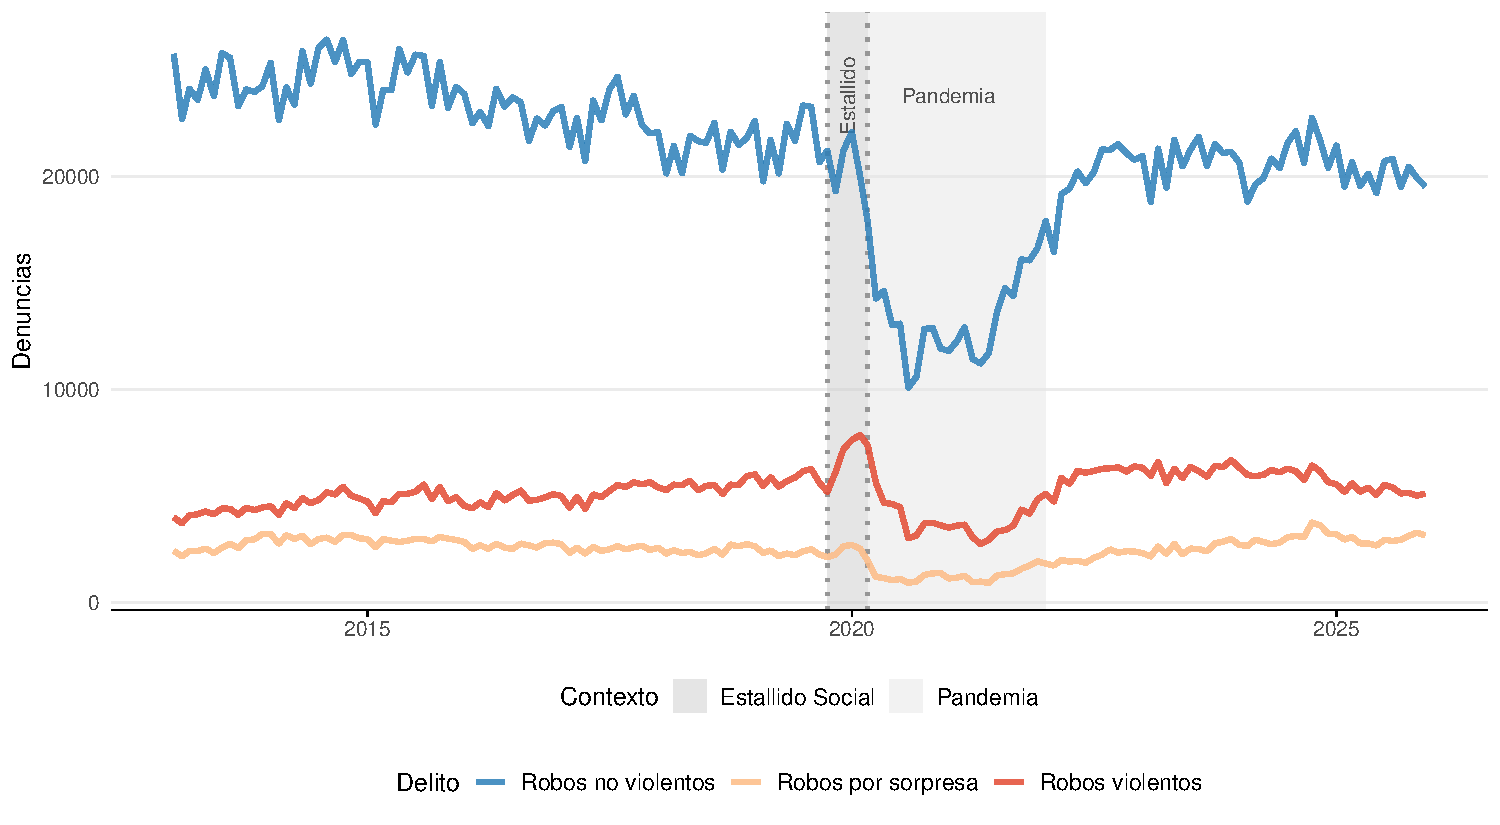
\includegraphics[width=\textwidth]{fig1_serie_mensual_nacional.pdf}
\caption{Serie mensual de casos policiales por categor\'ia C3, Chile 2013--2025.}
\label{fig:serie}
\tablenote{Las bandas sombreadas corresponden al estallido social (oct.\ 2019--feb.\
2020) y a la pandemia (mar.\ 2020--dic.\ 2021). Tasas por 100.000 habitantes.
Fuente: \citet{INE2026}; proyecciones INE Base 2024 (nivel nacional).}
\end{figure}

Las tasas anuales revelan el patr\'on estructural con mayor claridad. Los robos
violentos describieron una trayectoria ascendente desde 287 por 100.000
habitantes en 2013 hasta 372 en 2019, colapsaron a 222 durante la pandemia (2021), y
se recuperaron hasta alcanzar un nuevo m\'aximo de 377 en 2023 antes de iniciar una inflexi\'on a la baja en 2024--2025 (315 en 2025). Lo relevante es que, tras el m\'aximo hist\'orico de 2023, el Spline~4 captura una tendencia descendente que el modelo formaliza con IRR\,=\,0.868 ($p=0.057$), convergiendo hacia los niveles del inicio de la serie. Los robos no
violentos muestran un declive secular que abarca todo el per\'iodo: de cerca de 1.662
por 100.000 en 2013 a 1.253 en 2024, sin recuperaci\'on significativa
post-pandemia. Esta divergencia en trayectorias---robos violentos con nueva inflexi\'on descendente, no violentos en declive pronunciado y sostenido---es el mecanismo que genera
la paradoja del ratio creciente (Figura~\ref{fig:tasas}).

\begin{figure}[H]
\centering
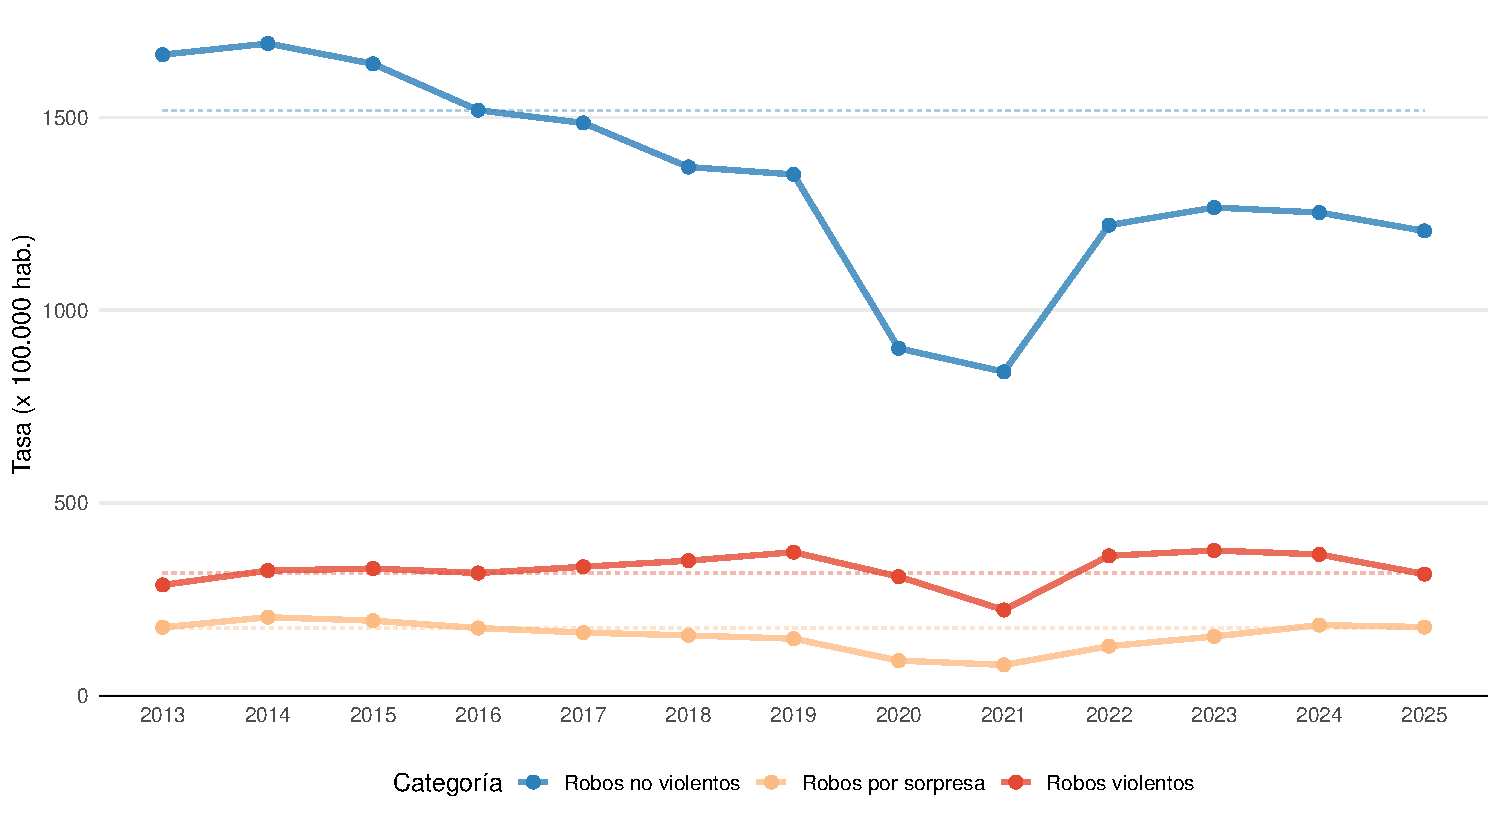
\includegraphics[width=\textwidth]{fig2_tasa_anual_nacional.pdf}
\caption{Tasas anuales de casos policiales por 100.000 habitantes, por categor\'ia C3,
Chile 2013--2025.}
\label{fig:tasas}
\tablenote{Las l\'ineas horizontales de referencia corresponden a la tasa del a\~no 2016
para cada categor\'ia. Fuente: \citet{INE2026}; proyecciones INE Base 2024
(nivel nacional).}
\end{figure}

Estas divergencias quedan cuantificadas en la Tabla~\ref{tab:descriptivo}, que sintetiza los estad\'isticos descriptivos por per\'iodo.

\begin{table}[H]
\centering
\caption{Estad\'isticos descriptivos por per\'iodo (robos violentos, panel regional)}
\label{tab:descriptivo}
\small
\begin{tabular}{lcccc}
\toprule
\textbf{Per\'iodo} & \textbf{N meses} & \textbf{Media} & \textbf{DE} & \textbf{Tasa media} \\
 & & (conteo) & (conteo) & (por 100.000) \\
\midrule
Pre-l\'inea base (2013--2015)       & 36 & 290.3 & 719.5 & 15.5 \\
L\'inea base (2016--sep.\ 2019)     & 45 & 330.0 & 875.2 & 14.9 \\
Estallido (oct.\ 2019--feb.\ 2020)  &  5 & 424.7 & 1200.8 & 17.4 \\
Pandemia (mar.\ 2020--dic.\ 2021)   & 22 & 247.2 & 698.4 & 10.3 \\
Post-pandemia (2022--2025)          & 48 & 366.6 & 939.1 & 16.3 \\
\bottomrule
\end{tabular}
\tablenote{Observaciones: panel de 16 regiones $\times$ n\'umero de meses indicado.
La tasa media es el promedio de las 16 regiones. Fuente: \citet{INE2026};
SERMIG; proyecciones INE Base 2017.}
\end{table}

Desagregando los datos emp\'iricos (Tabla~\ref{tab:cum}), los dos delitos que dominan los robos
violentos---el robo con intimidaci\'on (64.3\% del grupo) y el robo con
violencia (28.7\%)---registran tasas post-pandemia $-22.9\%$ y $-8.3\%$ por debajo del
per\'iodo de l\'inea base, respectivamente. En conjunto representan el 93\% del grupo
y su tendencia a la baja es el elemento m\'as robusto del an\'alisis descriptivo. El
robo de veh\'iculo con violencia (portonazo) aparece en el sistema con volumen sustancial solo desde 2020,
representando el 6.6\% del grupo en el per\'iodo completo; por tanto, su comparativa toma el 2020--2021 como l\'inea base
referencial natural. El \'unico delito con
crecimiento real sostenido es el secuestro expr\'es (retenci\'on de v\'ictimas para obtener rescate o extracci\'on),
con un incremento de 263\% entre per\'iodos---pero desde una base muy reducida (menos
del 0.1\% del grupo): 83 casos en 2022 frente a 283 en 2025. En los robos no violentos,
la ca\'ida es generalizada: la m\'as pronunciada corresponde al robo en lugar habitado
($-35.0\%$) y al hurto de 0.5 a 4 UTM ($-25.7\%$).

\begin{table}[H]
\centering
\caption{Composici\'on intra-categor\'ia: CUMs principales de la clasificaci\'on C3 (2013--2025)}
\label{tab:cum}
\footnotesize
\begin{tabular}{lrp{5cm}rrrr}
\toprule
\textbf{Cat.} & \textbf{CUM} & \textbf{Glosa} & \textbf{N total} & \textbf{\% grupo} & \textbf{Tasa base\textsuperscript{a}} & \textbf{$\Delta$\%\textsuperscript{b}} \\
\midrule
\multicolumn{7}{l}{\textit{C3.1 --- Robos violentos}} \\
 & 802 & Robo con intimidaci\'on        & 519.171 & 64.3 & 238.5 & $-$22.9 \\
 & 803 & Robo con violencia             & 232.073 & 28.7 &  97.7 & $-$8.3  \\
 & 867 & Robo veh\'iculo c/viol.\ (portonazo) & 53.130 & 6.6 & --\textsuperscript{c} & n.a. \\
 & 828 & Robo con violaci\'on           &   1.470 &  0.2 &  0.66 & $-$14.1 \\
 & 862 & Retenci\'on de v\'ictimas      &     992 &  0.1 &  0.24 & $+$263  \\
 & 827 & Robo con homicidio             &     320 &  0.0 &  0.10 & $+$55   \\
 & 861 & Robo con lesiones graves       &     175 &  0.0 &  0.09 & $+$17   \\
 & 829 & Robo c/castraci\'on/mutilaci\'on &   15  &  0.0 & 0.005 & $+$71   \\
\midrule
\multicolumn{7}{l}{\textit{C3.2 --- Robos por sorpresa}} \\
 & 804 & Robo por sorpresa (lanzazo)   & 382.445 & 100.0 & 158.2 & $-$8.0 \\
\midrule
\multicolumn{7}{l}{\textit{C3.3 --- Robos no violentos}} \\
 & 808 & Robo en lugar uso p\'ublico   & 739.657 & 22.7 & 317.3 & $-$18.9 \\
 & 809 & Robo en lugar habitado        & 589.940 & 18.1 & 268.9 & $-$35.0 \\
 & 847 & Hurto 4--40 UTM               & 544.015 & 16.7 & 235.5 & $-$15.4 \\
 & 810 & Robo en lugar no habitado     & 480.777 & 14.7 & 206.6 & $-$15.8 \\
 & 848 & Hurto 0.5--4 UTM              & 403.089 & 12.3 & 174.4 & $-$25.7 \\
 & 831 & Robo veh\'iculo sin violencia  & 350.990 & 10.8 & 137.0 & $-$4.8  \\
 & --- & Resto                          &    --- &  4.7 &   --- & variable \\
\bottomrule
\end{tabular}
\tablenote{\textsuperscript{a} Tasa promedio por 100.000 hab.\ en el per\'iodo de
l\'inea base (2016--2019). \textsuperscript{b} Cambio porcentual entre tasa base
(2016--2019) y tasa post-pandemia (2022--2025). \textsuperscript{c} El portonazo se
activa en el sistema con volumen significativo desde 2020; la tasa base no es
comparable. N total = casos policiales 2013--2025. Fuente: \citet{INE2026};
SERMIG; proyecciones INE Base 2017.}
\end{table}

El ratio mensual robos violentos/(violentos + no violentos), una vez desestacionalizado
y suavizado mediante una regresi\'on local polinomial (LOESS; \textit{locally estimated
scatterplot smoothing}), asciende de forma casi mon\'otona desde 14.7\% en abril de
2015 hasta un m\'aximo hist\'orico de 21.6\% en enero de 2024. El estimador LOESS ajusta
en cada punto una regresi\'on ponderada sobre los valores temporalmente m\'as pr\'oximos;
el par\'ametro \texttt{span}\,=\,0.2 equivale a utilizar el 20\% de las observaciones
como ventana de suavizado. Su funci\'on es exclusivamente descriptiva: revela la
tendencia subyacente filtrada del ruido estacional de corto plazo, sin constituir un
test de hip\'otesis formal; la curva resultante es consistente con ---pero conceptualmente
independiente de--- los quiebres formales del Bai-Perron. El algoritmo de Bai-Perron, seleccionando
$m=4$ quiebres por BIC, identifica cuatro inflexiones sucesivas: Q1 en abril de 2015
(14.7\%), Q2 en agosto de 2017 (17.1\%), Q3 en octubre de 2019 (18.4\%) y Q4 en enero
de 2024 (21.6\%). Cada quiebre marca un nuevo nivel del ratio, pero el mecanismo que
los sostiene no es el crecimiento de los robos violentos, sino la contracci\'on m\'as
pronunciada de los robos no violentos en el denominador. Esta paradoja---ratio creciente
con volumen absoluto decreciente---constituye el hallazgo central del trabajo
(Figura~\ref{fig:ratio}).

\begin{figure}[H]
\centering
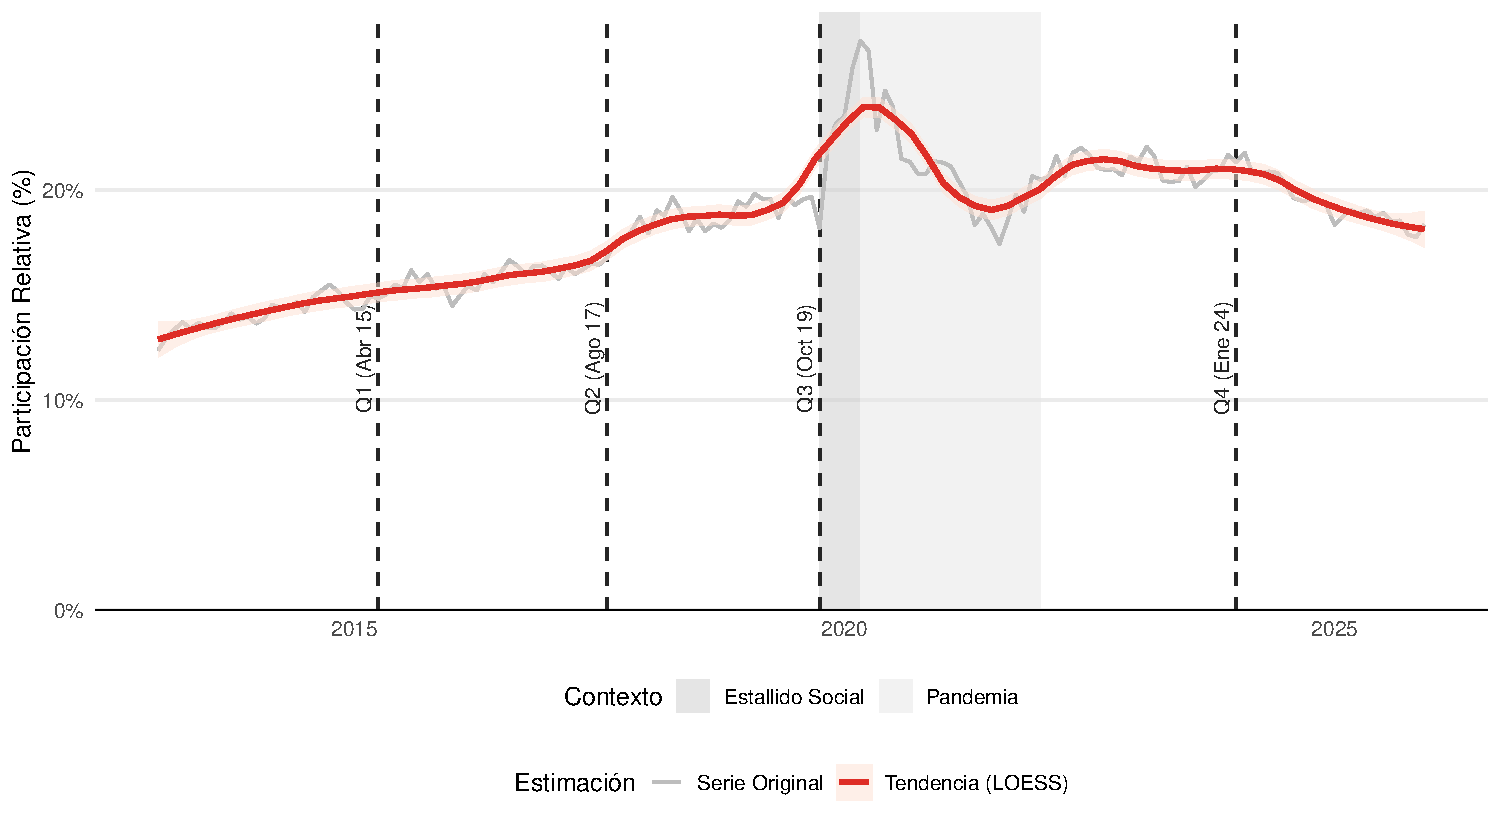
\includegraphics[width=\textwidth]{fig3_ratio_violentos_mensual.pdf}
\caption{Ratio mensual robos violentos/(violentos + no violentos) con quiebres de
Bai-Perron.}
\label{fig:ratio}
\tablenote{Las l\'ineas verticales discontinuas marcan los cuatro quiebres \'optimos por
BIC: Q1 = abr.\ 2015 (14.7\%); Q2 = ago.\ 2017 (17.1\%); Q3 = oct.\ 2019 (18.4\%);
Q4 = ene.\ 2024 (21.6\%). La serie est\'a desestacionalizada. Fuente: \citet{INE2026}.}
\end{figure}

\subsection{Estimaci\'on de la tendencia secular}
\label{sub:inferencial}

La Tabla~\ref{tab:poisson} reporta los resultados del modelo Poisson-QMLE para las
tres categor\'ias C3. Para los robos violentos, el estallido social produjo un aumento
transitorio de 15.5\% (IRR\,=\,1.155; $p<0.001$), consistente con la hip\'otesis de
que el clima de protesta facilit\'o delitos de confrontaci\'on directa. Los robos por
sorpresa aumentaron 6.9\% (IRR\,=\,1.069; $p<0.001$). En contraste, los robos no
violentos no reaccionaron al estallido (IRR\,=\,0.996; $p=0.761$): su din\'amica
responde a factores estructurales de oportunidad, no a la conflictividad social. La
pandemia produjo una ca\'ida generalizada y significativa: $-34.9\%$ en violentos
(IRR\,=\,0.651), $-42.4\%$ en sorpresa (IRR\,=\,0.576) y $-35.3\%$ en no violentos
(IRR\,=\,0.647). La mayor intensidad de la ca\'ida para sorpresa refleja su dependencia
de la aglomeraci\'on urbana, bloqueada por las cuarentenas.

El componente m\'as informativo es la trayectoria del spline. Para los robos violentos,
los primeros tres tramos muestran crecimiento moderado---Spline~1 (2013--2016):
IRR\,=\,1.178, $p=0.201$; Spline~2 (2016--2019): IRR\,=\,1.136, $p=0.087$;
Spline~3 (2019--2022): IRR\,=\,1.187, $p<0.001$. El resultado m\'as relevante es el
Spline~4, que captura el per\'iodo septiembre 2022--diciembre 2025: IRR\,=\,0.868
($p=0.057$ por WCB), indicando una inflexi\'on descendente que comienza a emerger
estad\'isticamente. Con $G=16$ clusters, un p-valor de 0.057 es evidencia sugestiva;
su consistencia con el an\'alisis descriptivo y con los placebos fortalece la
interpretaci\'on de declive real.

Para los robos no violentos, el declive es robusto, mon\'otono y significativo en todos
los tramos: los cuatro coeficientes del spline son negativos y altamente significativos,
con Spline~4 mostrando IRR\,=\,0.648 ($p<0.001$), una reducci\'on del 35.2\% respecto
del nivel inicial. Esta tendencia comenz\'o antes de la pandemia y se profundiz\'o a lo
largo de todo el horizonte observado, coherente con cambios estructurales en las
actividades rutinarias---expansi\'on del comercio electr\'onico y seguridad residencial.
Para los robos por sorpresa, la ca\'ida secular domina en los tramos iniciales
(Spline~1: IRR\,=\,0.668; Spline~2: IRR\,=\,0.635), con estabilizaci\'on en el per\'iodo
reciente (Spline~4: IRR\,=\,0.861, $p=0.574$). La divergencia entre categor\'ias
confirma el valor de la clasificaci\'on tricot\'omica: los tres tipos de robo siguen
trayectorias cualitativamente distintas.

\begin{table}[H]
\centering
\caption{Modelo Poisson-QMLE con Wild Cluster Bootstrap: resultados principales (C3)}
\label{tab:poisson}
\footnotesize
\begin{tabular}{l@{\hskip 3mm}ccc@{\hskip 4mm}ccc@{\hskip 4mm}ccc}
\toprule
 & \multicolumn{3}{c}{\textbf{Robos violentos}} & \multicolumn{3}{c}{\textbf{Robos sorpresa}} & \multicolumn{3}{c}{\textbf{No violentos}} \\
\cmidrule(lr){2-4}\cmidrule(lr){5-7}\cmidrule(lr){8-10}
\textbf{T\'ermino} & IRR & IC 95\% & $p$ & IRR & IC 95\% & $p$ & IRR & IC 95\% & $p$ \\
\midrule
$D^{\text{est}}$ & 1.155 & [1.119, 1.192] & $<$.001 & 1.069 & [1.031, 1.108] & $<$.001 & 0.996 & [0.971, 1.022] & .761 \\
$D^{\text{pan}}$ & 0.651 & [0.621, 0.682] & $<$.001 & 0.576 & [0.547, 0.606] & $<$.001 & 0.647 & [0.628, 0.665] & $<$.001 \\
\midrule
Spline 1    & 1.178 & [0.917, 1.513] & .201 & 0.668 & [0.619, 0.722] & $<$.001 & 0.718 & [0.673, 0.767] & $<$.001 \\
Spline 2    & 1.136 & [0.982, 1.315] & .087 & 0.635 & [0.462, 0.873] & .005 & 0.685 & [0.568, 0.826] & $<$.001 \\
Spline 3    & 1.187 & [1.116, 1.264] & $<$.001 & 0.968 & [0.634, 1.480] & .882 & 0.656 & [0.570, 0.754] & $<$.001 \\
\textbf{Spline 4} & \textbf{0.868} & \textbf{[0.751, 1.004]} & \textbf{.057} & 0.861 & [0.511, 1.450] & .574 & \textbf{0.648} & \textbf{[0.580, 0.723]} & $<$.001 \\
\midrule
Obs. & 2.496 & & & 2.496 & & & 2.496 & & \\
\bottomrule
\end{tabular}
\tablenote{IRR = exp($\hat{\beta}$). IC 95\% por inversi\'on del WCB (pesos de Webb,
$B=9{,}999$, $G=16$). $D^{\text{est}}$: dummy estallido social (oct.\ 2019--feb.\
2020). $D^{\text{pan}}$: dummy pandemia (mar.\ 2020--dic.\ 2021). Spline~1--4: spline
c\'ubico restringido con nodos en P25 ($\approx$ mar.\ 2016), P50 ($\approx$ jun.\ 2019)
y P75 ($\approx$ sep.\ 2022). Todos los modelos incluyen efectos fijos regionales y
dummies mensuales de estacionalidad. Offset: $\log$(poblaci\'on mensual corregida).}
\end{table}

\subsection{Heterogeneidad regional y quiebres CUSUM}
\label{sub:regional}

Los tests CUSUM-GLM revelan que el cambio estructural en los robos violentos es real pero
temporalmente heterog\'eneo: 12 de 16 regiones presentan quiebre significativo
(p-FDR\,<\,0.05), pero en tres momentos distintos que responden a l\'ogicas locales
diferentes (Tabla~\ref{tab:cusum}).

El primer grupo, de quiebre pre-pandemia, comprende las regiones de la macrozona Sur
(Maule: abril 2017; Biob\'io: agosto 2018; La Araucan\'ia: julio 2018) y Magallanes
(agosto 2017). Estas inflexiones preceden en m\'as de dos a\~nos al estallido social,
lo que indica procesos locales independientes del shock nacional: din\'amicas de
migraci\'on interna, expansi\'on de econom\'ias il\'icitas territoriales y
reconfiguraci\'on de redes criminales en el sur. El segundo grupo, de quiebre durante
la pandemia y la reactivaci\'on, agrupa a la mayor\'ia de las regiones---Regi\'on
Metropolitana (julio 2020), Atacama (agosto 2021), O'Higgins (septiembre 2021), Coquimbo
(septiembre 2021), Arica y Parinacota (julio 2021) y \~Nuble (agosto 2021)---con
inflexiones concentradas entre julio de 2020 y septiembre de 2021. La combinaci\'on de
restricciones de movilidad y posterior reactivaci\'on reorganiz\'o los patrones
delictuales de manera suficientemente profunda como para generar quiebres
estad\'isticamente detectables. El tercer grupo, de quiebre tard\'io, corresponde
exclusivamente a Tarapac\'a (agosto 2023): la intensidad migratoria desde la frontera
norte y la reconfiguraci\'on de rutas del crimen organizado explican este desfase.
Cuatro regiones---Antofagasta, Valpara\'iso, Los Lagos y Los R\'ios---no muestran
evidencia de quiebre significativo.

\begin{table}[H]
\centering
\caption{Tests CUSUM-GLM: quiebre estructural en robos violentos por regi\'on}
\label{tab:cusum}
\footnotesize
\begin{tabular}{llccc}
\toprule
\textbf{Regi\'on} & \textbf{Macrozona} & \textbf{p-valor} & \textbf{p-FDR} & \textbf{Quiebre estimado} \\
\midrule
R15 --- Arica y Parinacota & Norte   & $<$.001  & $<$.001 & Jul.\ 2021 \\
R8 --- Biob\'io            & Sur     & $<$.001  & $<$.001 & Ago.\ 2018 \\
R9 --- La Araucan\'ia      & Sur     & $<$.001  & $<$.001 & Jul.\ 2018 \\
R7 --- Maule               & Centro  & $<$.001  & $<$.001 & Abr.\ 2017 \\
R3 --- Atacama             & Norte   & $<$.001  & $<$.001 & Ago.\ 2021 \\
R6 --- O'Higgins           & Centro  & $<$.001  & $<$.001 & Sep.\ 2021 \\
R13 --- Metropolitana      & RM      & $<$.001  & $<$.001 & Jul.\ 2020 \\
R11 --- Ays\'en            & Austral & .001     & .001    & Feb.\ 2016 \\
R12 --- Magallanes         & Austral & .001     & .003    & Ago.\ 2017 \\
R1 --- Tarapac\'a          & Norte   & .003     & .005    & Ago.\ 2023 \\
R4 --- Coquimbo            & Norte   & .006     & .009    & Sep.\ 2021 \\
R16 --- \~Nuble            & Sur     & .016     & .022    & Ago.\ 2021 \\
\midrule
R2 --- Antofagasta         & Norte   & .194     & .207    & (n.s.) \\
R5 --- Valpara\'iso        & Centro  & .334     & .334    & (n.s.) \\
R10 --- Los Lagos          & Sur     & .176     & .201    & (n.s.) \\
R14 --- Los R\'ios         & Sur     & .144     & .177    & (n.s.) \\
\bottomrule
\end{tabular}
\tablenote{Test supremo de puente browniano sobre el proceso emp\'irico de fluctuaci\'on
del GLM regional. p-FDR: correcci\'on Benjamini-Hochberg sobre los 16 p-valores. El
quiebre estimado corresponde al mes de mayor acumulaci\'on del estad\'istico CUSUM.}
\end{table}

La trayectoria acumulada del residuo en cada regi\'on muestra c\'omo el proceso supera
los l\'imites cr\'iticos al 95\% en momentos distintos, evidenciando la ausencia de un
shock nacional sincr\'onico (Figura~\ref{fig:cusum}). Geogr\'aficamente, los quiebres
pre-pandemia se concentran en el sur, mientras los de pandemia y reactivaci\'on se
distribuyen por el centro y norte del pa\'is (Figura~\ref{fig:mapatasa}).

\begin{figure}[H]
\centering
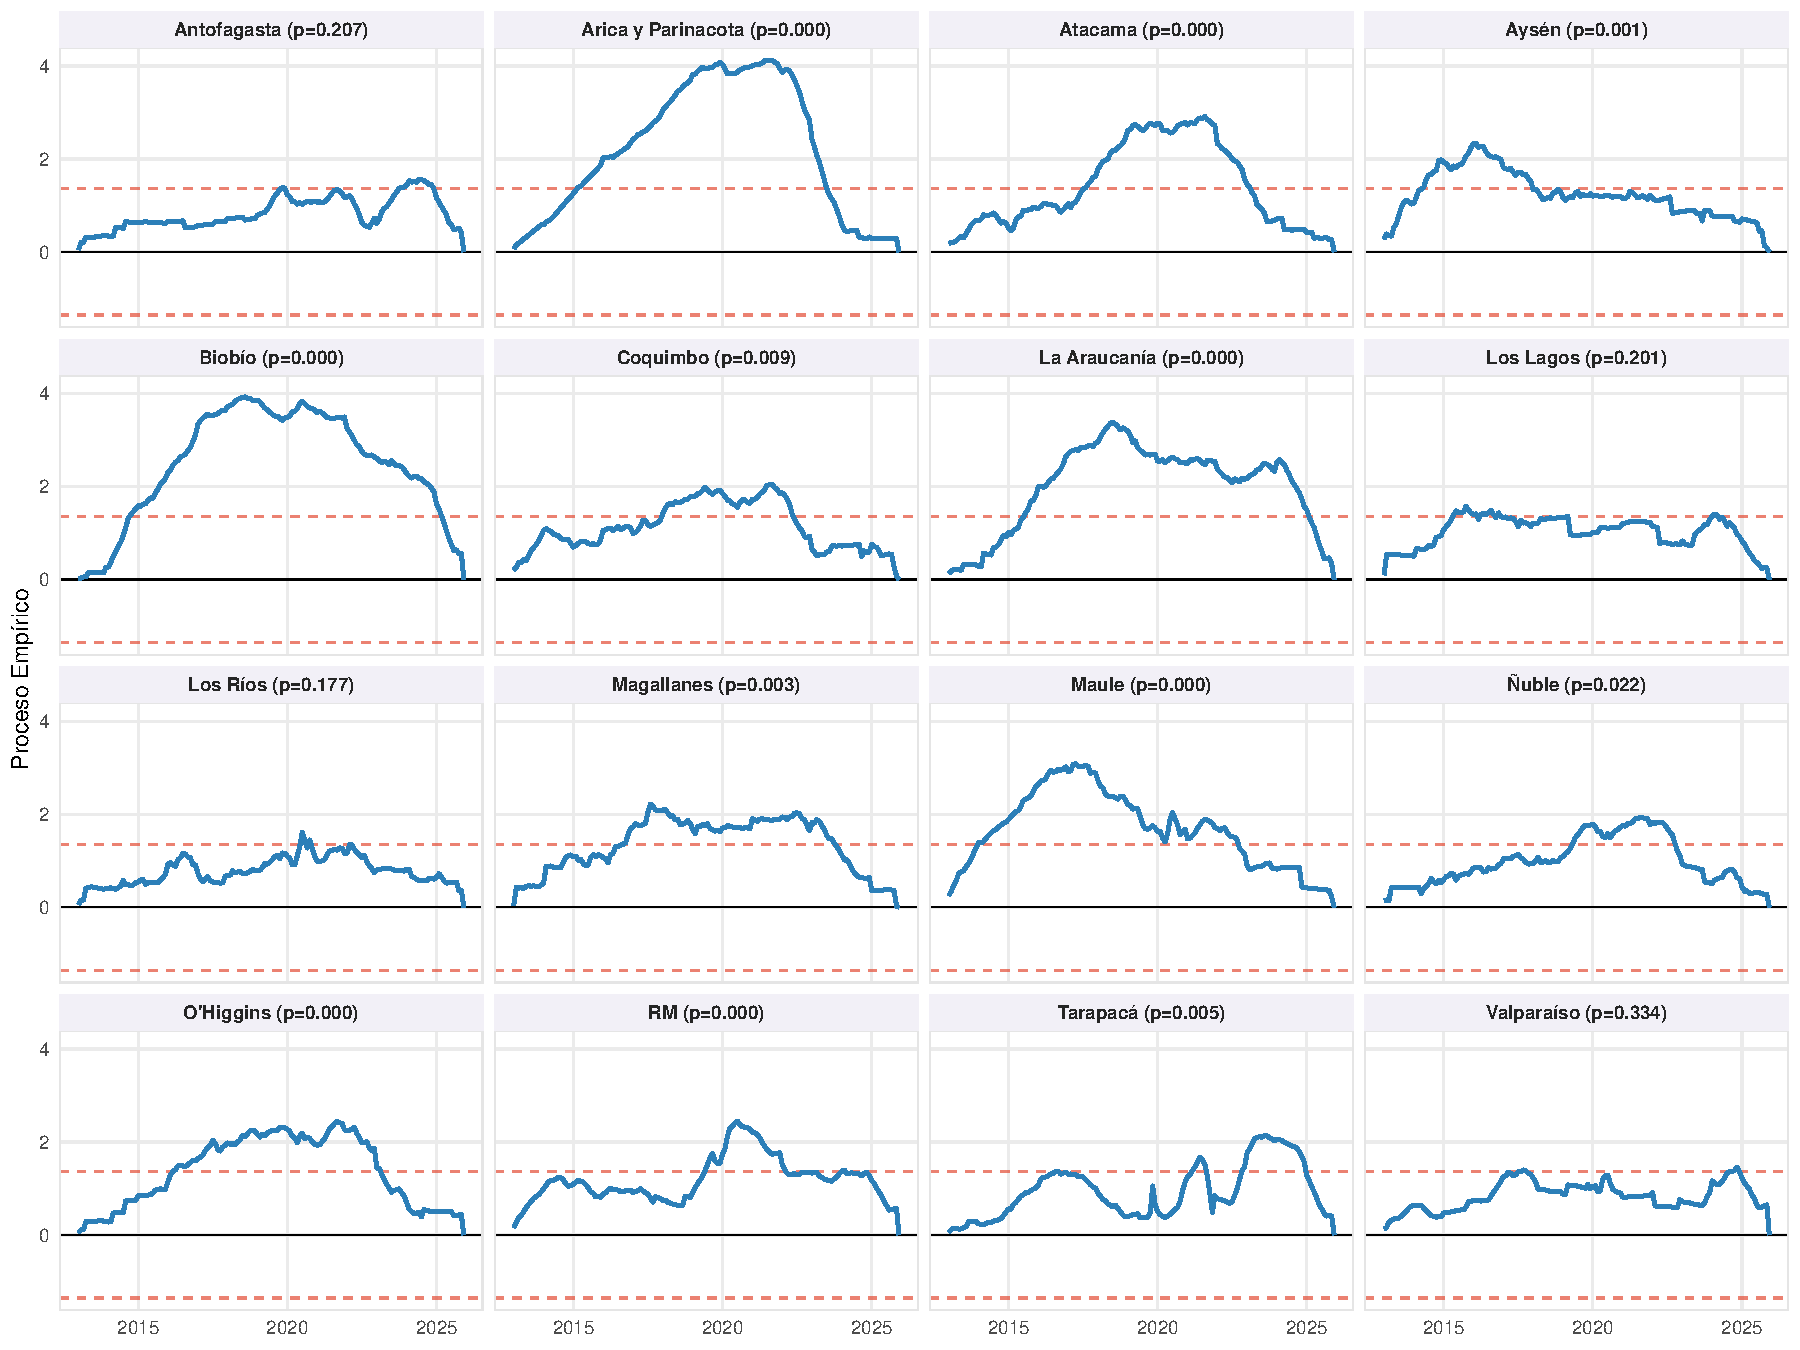
\includegraphics[width=\textwidth]{fig4_cusum_regional_facet.pdf}
\caption{Procesos CUSUM-GLM para las 16 regiones (robos violentos, C3.1).}
\label{fig:cusum}
\tablenote{Las bandas corresponden a los l\'imites cr\'iticos al 95\% del proceso de
puente browniano. Regiones con quiebre significativo (p-FDR\,<\,0.05) se destacan en
rojo. Fuente: \citet{INE2026}; SERMIG; proyecciones INE Base 2017.}
\end{figure}
La comparaci\'on directa entre el Spline~1 (2013--2016) y el Spline~4 (2022--2025) muestra heterogeneidad regional sustantiva en la tasa de robos violentos (Figura~\ref{fig:mapatasa}).
Las regiones del norte, en particular Arica y Parinacota, exhiben los mayores incrementos entre ambos per\'iodos, coherente con la presi\'on migratoria y los quiebres CUSUM identificados. Las regiones del sur con quiebres tempranos tienden a mostrar diferencias inter-per\'iodo m\'as modestas.

\begin{figure}[H]
\centering
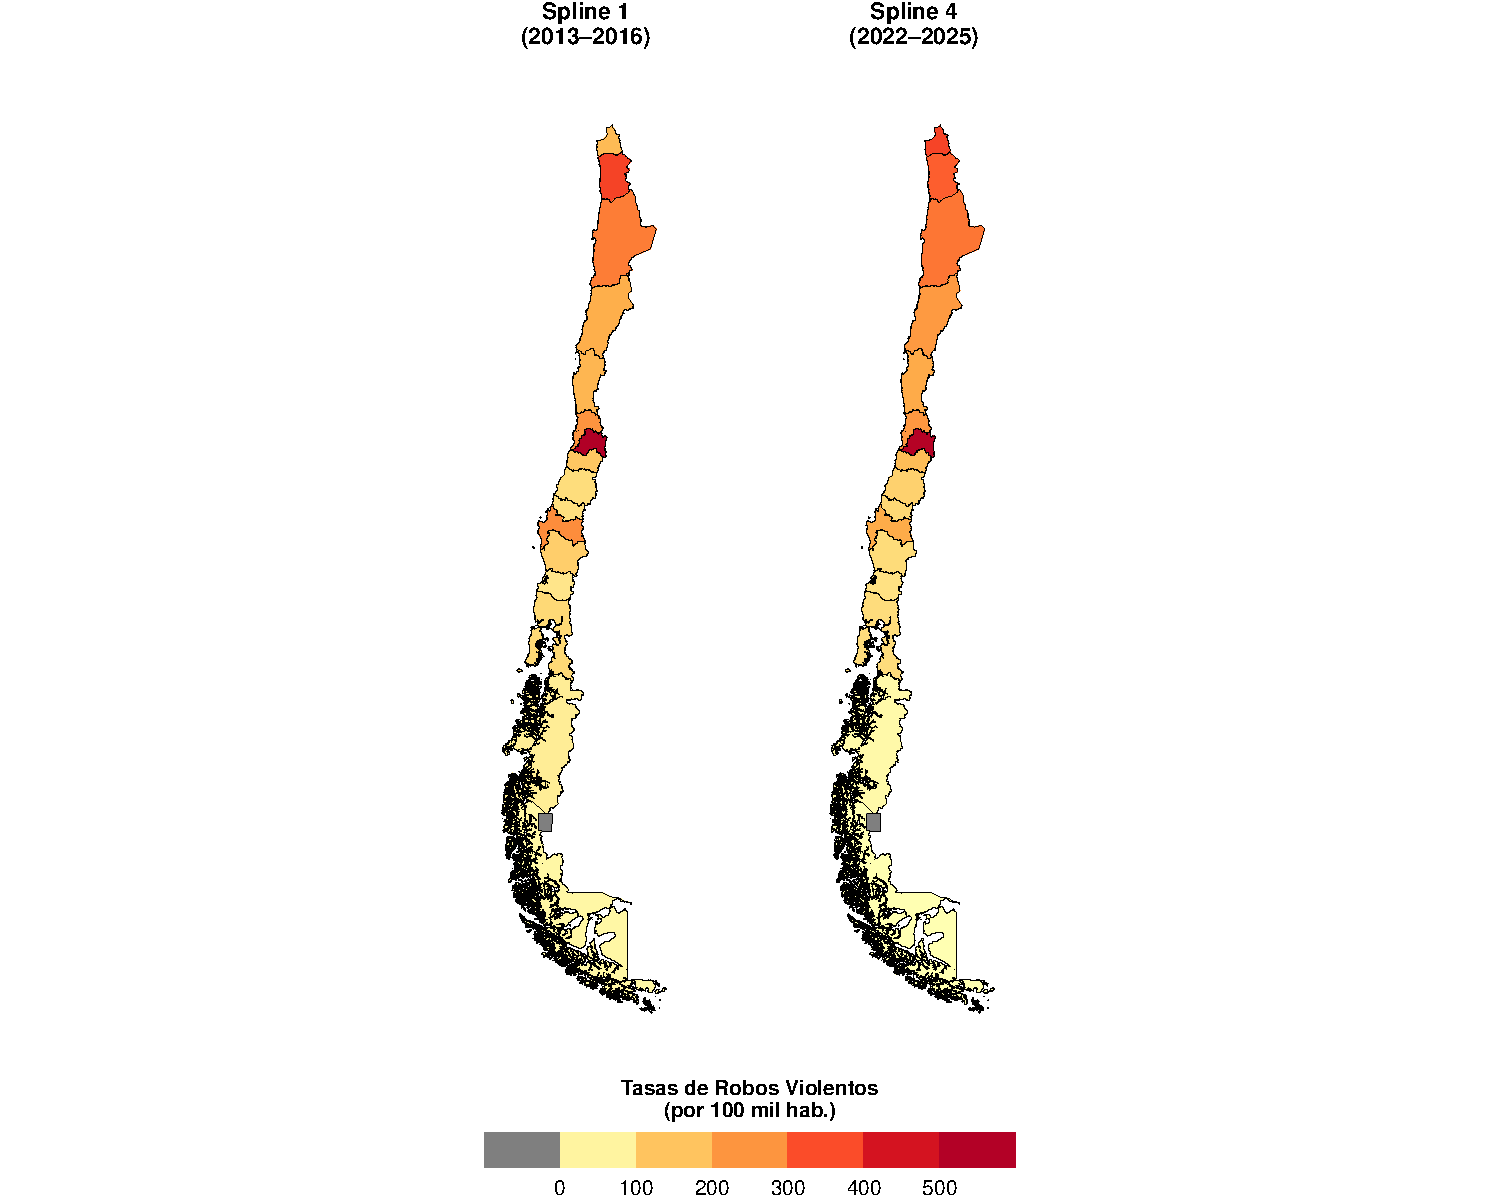
\includegraphics[width=0.88\textwidth]{map1_tasa_sidebyside.pdf}
\caption{Tasas de robos violentos por regi\'on: Spline~1 (2013--2016) versus Spline~4 (2022--2025), por 100.000 hab.}
\label{fig:mapatasa}
\tablenote{Promedio del per\'iodo en cada regi\'on. Fuente: \citet{INE2026};
SERMIG; proyecciones INE Base 2017.}
\end{figure}

El modelo de interacciones macrozona $\times$ spline (Ap\'endice~\ref{ap:macro}) revela que la tendencia de largo plazo difiere significativamente entre zonas geogr\'aficas (test de Wald conjunto: $p<0.001$). En el primer tramo (Spline~1, 2013--2016), la Regi\'on Metropolitana exhibe el mayor crecimiento relativo (IRR\,=\,2.68 respecto de Austral), seguida por la macrozona Centro (IRR\,=\,1.82). En el Spline~2 (2016--2019), la macrozona Norte lidera con el IRR m\'as elevado (3.94), coherente con la presi\'on migratoria acumulada y el quiebre CUSUM identificado en Arica y Parinacota (julio de 2021, con un rezago que sugiere acumulaci\'on latente). En el Spline~3 (2019--2022), el Centro alcanza su mayor dinamismo (IRR\,=\,3.57). En el Spline~4 (2022--2025), sin embargo, todas las interacciones convergen hacia la unidad---Norte: IRR\,=\,1.08; Centro: 1.37; Sur: 1.00---lo que indica que la inflexi\'on descendente reciente es un fen\'omeno de alcance nacional y no un artefacto de ninguna zona en particular.

\subsection{Validaci\'on mediante placebos}
\label{sub:placebos}

Tres modelos de validaci\'on proveen evidencia convergente sobre la especificidad y
potencia del modelo principal (Tabla~\ref{tab:placebos}).

El placebo negativo (P1, cuasidelito vehicular) refleja la reactivaci\'on de la
actividad vial post-pandemia: todos sus tramos del spline son positivos y significativos,
con el Spline~4 mostrando IRR\,=\,2.036 ($p<0.001$). El mismo modelo que detect\'o
inflexi\'on negativa en robos violentos captura aqu\'i un crecimiento pronunciado. Esto
descarta la posibilidad de que la especificaci\'on subvalore sistem\'aticamente la
actividad en el per\'iodo m\'as reciente: el resultado negativo del Spline~4 en robos
violentos no es un artefacto del modelo.

El placebo positivo (P2, homicidios dolosos CCH) ofrece la contraprueba directa: si la
violencia real est\'a aumentando, el modelo debe detectarlo. Y as\'i ocurre. Los
Splines~2 y 3 registran IRR\,=\,2.746 y 3.612 ($p<0.001$ en ambos), capturando el
aumento real de los homicidios entre 2016 y 2022. En el Spline~4, los homicidios
arrojan IRR\,=\,2.061 ($p<0.001$)---a\'un en territorio de crecimiento, a diferencia
de los robos violentos que muestran inflexi\'on descendente. Esta divergencia entre
homicidios (crecientes en Spline~4) y robos violentos (decrecientes) no puede atribuirse
a un problema de especificaci\'on: el modelo detecta de manera diferencial din\'amicas
opuestas, lo que valida su capacidad discriminante. Adicionalmente, la triangulaci\'on de los homicidios a nivel de macrozonas revela que esta alza letal no es espacialmente sim\'etrica ni sincr\'onica. Mientras que la macrozona Austral no exhibe un quiebre significativo en su serie, la macrozona Norte experiment\'o el aumento m\'as agudo y temprano durante el per\'iodo 2016--2019 (Spline~2: IRR\,=\,2.25, $p<0.001$). En contraste, las macrozonas Centro, RM y Sur muestran una trayectoria de crecimiento sostenido prolongada, alcanzando su mayor velocidad de expansi\'on relativa entre 2019 y 2022 (Spline~3 con coeficientes IRR superiores a 2.65). Esto indica que, mientras los robos violentos retroceden nacionalmente tras la pandemia, el recrudecimiento de la letalidad tuvo anclajes y cronolog\'ias regionales diferenciadas.

La triangulaci\'on con los homicidios confirmados del CPHDV provee el punto de
comparaci\'on m\'as robusto frente a la cifra negra. Los registros anuales muestran un
crecimiento desde aproximadamente 900 homicidios confirmados en 2018 hasta un m\'aximo
de 1.330 en 2022, seguido de un descenso sostenido: 1.249 en 2023, 1.209 en 2024 y
1.091 en 2025. El Spline~4 para el CPHDV no es estad\'isticamente significativo
(IRR\,=\,1.075, $p=0.530$), indicando que el crecimiento de la violencia letal se
desaceler\'o en el per\'iodo m\'as reciente. La moderaci\'on paralela en homicidios
confirmados y en robos violentos traza un cuadro coherente: ambos indicadores apuntan
a un techo alcanzado en torno a 2022 y una desaceleraci\'on posterior.

\begin{table}[H]
\centering
\caption{Placebos y validaci\'on externa: modelos Poisson-QMLE}
\label{tab:placebos}
\footnotesize
\begin{tabular}{lccc@{\hskip 4mm}cc@{\hskip 4mm}cc}
\toprule
 & \multicolumn{3}{c}{\textbf{P1: Cuasidelito vehicular}} & \multicolumn{2}{c}{\textbf{P2: Homicidios CCH}} & \multicolumn{2}{c}{\textbf{CPHDV (confirmados)}} \\
\cmidrule(lr){2-4}\cmidrule(lr){5-6}\cmidrule(lr){7-8}
\textbf{T\'ermino} & IRR & IC 95\% & $p$ & IRR & $p$ & IRR & $p$ \\
\midrule
$D^{\text{est}}$ & 1.105 & [0.989, 1.234] & .078 & 1.144 & .097 & 1.046 & .763 \\
$D^{\text{pan}}$ & 0.874 & [0.750, 1.020] & .087 & 1.009 & .949 & 0.871 & .367 \\
\midrule
Spline 1 &  9.080 & [3.09, 26.70] & $<$.001 & 1.300 & .096 & 1.562 & .001 \\
Spline 2 &  3.820 & [1.85,  7.90] & $<$.001 & 2.746 & $<$.001 & 1.430 & $<$.001 \\
Spline 3 & 48.380 & [6.78, 345.4] & $<$.001 & 3.612 & $<$.001 & 1.774 & .113 \\
\textbf{Spline 4} & \textbf{2.036} & [1.397, 2.969] & $<$.001 & \textbf{2.061} & $<$.001 & 1.075 & .530 \\
\bottomrule
\end{tabular}
\tablenote{P1 y P2 se estiman sobre el panel regional (16 regiones $\times$ 156 meses);
CPHDV sobre serie nacional (2018--2025, nodos propios). Los IRR grandes de P1 en
Spline~3 reflejan la normalizaci\'on del tr\'afico post-pandemia en escala logar\'itmica.
Inferencia: WCB (pesos de Webb, $B=9{,}999$) para P1 y P2; errores QMLE est\'andar para
CPHDV.}
\end{table}




% =========================================================
\section{An\'alisis de robustez}
\label{sec:robustez}
% =========================================================

El an\'alisis de robustez examina la estabilidad del resultado principal bajo seis ejes de variaci\'on. Los ejes R1, R3 y R5 eval\'uan la sensibilidad al denominador y a la parametrizaci\'on del trend; R6 reemplaza las denuncias por las detenciones en flagrancia para explorar la disociaci\'on entre victimizaci\'on ciudadana y actividad policial; R7 flexibiliza el spline; y las clasificaciones dicot\'omicas C1 y C2 ---reportadas en el Ap\'endice~\ref{ap:clasif}--- constituyen una dimensi\'on adicional de sensibilidad de clasificaci\'on.

Estas divergencias quedan cuantificadas en la Tabla~\ref{tab:robustez}, que reporta el coeficiente de tendencia del modelo bajo seis
especificaciones alternativas para robos violentos. Las especificaciones R1 (offset
libre), R3 (sin correcci\'on SERMIG) y R5 (nodos te\'oricos en 2016, 2019 y 2022)
producen coeficientes positivos y no significativos para el Spline~1 (2013--2016),
coherentes con el resultado principal. Que los nodos te\'oricos (R5) produzcan un
resultado diferente al de los nodos agn\'osticos refuerza la justificaci\'on metodol\'ogica:
la ubicaci\'on de los nodos importa, y el enfoque agn\'ostico es preferible a imponer
una estructura te\'orica que puede no coincidir con los datos.

La especificaci\'on R6, con detenciones en flagrancia como variable dependiente en lugar
de casos policiales totales, produce un coeficiente negativo y significativo
(IRR\,=\,0.878, $p=0.017$). Esto no contradice el resultado principal: las detenciones
responden adicionalmente a la proactividad policial---operativos, patrullajes focalizados,
prioridades institucionales---lo que genera una serie con din\'amica propia, distinta
de la victimizaci\'on ciudadana. La especificaci\'on R7 (spline m\'as flexible, df\,=\,5)
produce un coeficiente positivo y significativo (IRR\,=\,1.239, $p=0.006$).

\begin{table}[H]
\centering
\caption{An\'alisis de robustez: coeficiente de tendencia bajo especificaciones
alternativas (robos violentos, C3.1)}
\label{tab:robustez}
\small
\begin{tabular}{llccc}
\toprule
\textbf{ID} & \textbf{Especificaci\'on} & \textbf{Estimador} & \textbf{IRR} & $p$ \\
\midrule
Principal & Modelo base (spline P25/P50/P75, WCB) & 0.163 & 1.178 & .201 \\
\midrule
R1 & Offset libre (pob.\ como regresor)    & 0.075 & 1.078 & .546 \\
R3 & Sin correcci\'on SERMIG               & 0.214 & 1.238 & .119 \\
R5 & Nodos te\'oricos (2016, 2019, 2022)   & 0.168 & 1.183 & .160 \\
R6 & Detenciones como variable dependiente & $-$0.130 & 0.878 & .017 \\
R7 & Spline m\'as flexible (df\,=\,5)      & 0.214 & 1.239 & .006 \\
\bottomrule
\end{tabular}
\tablenote{El estimador reportado corresponde al Spline~1 del modelo (tendencia en el
per\'iodo 2013--2016). La inflexi\'on reciente (Spline~4: IRR\,=\,0.868, $p=0.057$) se
reporta en la Tabla~\ref{tab:poisson}. Todas las especificaciones incluyen dummies de
estallido/pandemia, efectos fijos regionales y estacionalidad mensual.}
\end{table}

La Tabla~\ref{tab:sensipop} examina la sensibilidad al denominador de poblaci\'on
irregular bajo factores de inflaci\'on demogr\'afica $k \in \{1.00, 1.05, 1.10,
1.15, 1.20\}$ aplicados a regiones de alta inmigraci\'on. El estimador y el IRR
permanecen id\'enticos en todos los escenarios (estimador\,=\,0.163; IRR\,=\,1.178),
con variaciones m\'inimas en el error est\'andar que no afectan la significancia. La
invariancia se explica porque el factor $k$ desplaza el offset uniformemente, afectando
el intercepto pero no los coeficientes de tendencia. Los resultados son por tanto robustos
a cualquier supuesto plausible sobre la poblaci\'on irregular no capturada por SERMIG.

\begin{table}[H]
\centering
\caption{Sensibilidad al denominador irregular: factor de inflaci\'on $k$ sobre
poblaci\'on corregida (robos violentos)}
\label{tab:sensipop}
\small
\begin{tabular}{ccccc}
\toprule
\textbf{Factor $k$} & \textbf{Estimador} & \textbf{EE (WCB)} & \textbf{IRR} & $p$ \\
\midrule
1.00 & 0.163 & 0.123 & 1.178 & .185 \\
1.05 & 0.163 & 0.130 & 1.178 & .210 \\
1.10 & 0.163 & 0.128 & 1.178 & .202 \\
1.15 & 0.163 & 0.125 & 1.178 & .193 \\
1.20 & 0.163 & 0.129 & 1.178 & .206 \\
\bottomrule
\end{tabular}
\tablenote{$k$ = factor de inflaci\'on aplicado a la poblaci\'on corregida de regiones
de alta inmigraci\'on (Tarapac\'a, Antofagasta, Arica y Parinacota, Regi\'on
Metropolitana). La invariancia del estimador y el IRR confirma que los resultados son
independientes de los supuestos sobre la poblaci\'on irregular.}
\end{table}


% =========================================================
\section{Discusi\'on}
\label{sec:discusion}
% =========================================================

La evidencia presentada sugiere que el debate p\'ublico sobre la ``crisis de seguridad''
en Chile captura algo real, pero lo describe de manera inexacta. Lo que existe es un
cambio cualitativo en la composici\'on de la delincuencia patrimonial: hoy una mayor
fracci\'on de los robos implica confrontaci\'on directa con la v\'ictima, aunque el
n\'umero absoluto de esos robos sea menor que en 2019. Este cambio compositivo es
estad\'isticamente robusto---el ratio robos violentos/total alcanz\'o un m\'aximo
hist\'orico de 21.6\% en enero de 2024, confirmado por cuatro quiebres sucesivos de
Bai-Perron y por la divergencia en los splines entre categor\'ias---pero su mecanismo
es el declive m\'as acelerado de los robos no violentos, no el aumento de los robos
violentos.

La l\'ogica del mecanismo es plausible desde la teor\'ia de las actividades rutinarias.
La expansi\'on del comercio electr\'onico y las plataformas de despacho a domicilio
reducen la circulaci\'on de bienes f\'isicos en el espacio p\'ublico. La mayor seguridad
residencial---proliferaci\'on de rejas, c\'amaras y alarmas---reduce la rentabilidad del
robo en domicilios y espacios no habitados. Los delitos que requieren coerci\'on directa
son menos sensibles a estas barreras: el delincuente que usa intimidaci\'on o violencia
enfrenta a su v\'ictima y no depende de condiciones de ausencia o desprotegi\'on. El
resultado es que los robos sin confrontaci\'on desaparecen m\'as r\'apido que aquellos
que los requieren, elevando el ratio incluso mientras el volumen total cae.

Pese al cuadro general de estabilizaci\'on en el volumen de robos violentos, dos
fen\'omenos emergentes exigen atenci\'on. El primero es la retenci\'on de
v\'ictimas: aunque representa menos del 0.1\% del grupo, creci\'o 263\% entre los
per\'iodos comparados, con 83 casos en 2022 y 283 en 2025. Este fen\'omeno responde a
una l\'ogica de crimen organizado---coerci\'on para transferencias bancarias---que
exige respuestas de pol\'itica diferenciadas. El segundo es el nivel de los homicidios
dolosos: pese al descenso posterior a 2022, los 1.091 homicidios confirmados de 2025
se mantienen sustancialmente por encima de los niveles previos al estallido social.

La distinci\'on entre volumen y composici\'on tiene consecuencias directas para el
dise\~no de pol\'itica. Una respuesta de volumen---mayor presencia policial para reducir
el total de hechos---no est\'a bien orientada si la din\'amica es compositiva. La
evidencia sugiere que las intervenciones deben focalizarse en los fen\'omenos emergentes
de alta lesividad: estrategias de protecci\'on de la banca y los canales de pago digital
frente al secuestro expr\'es, y desarticulaci\'on sostenida de estructuras de crimen
organizado vinculadas a la violencia letal.

Cuatro limitaciones deben considerarse. El efecto de la Comisaria Virtual sobre la
propensi\'on a denunciar no puede controlarse directamente, dado que los registros CCH
no identifican el canal de denuncia. El portonazo se activa con volumen significativo
solo desde 2020, lo que limita la historia comparable de este c\'odigo. El n\'umero
reducido de clusters ($G=16$) hace que el p-valor del Spline~4 de robos violentos
($p=0.057$) deba interpretarse con cautela, aunque su consistencia con los placebos
y el an\'alisis descriptivo atenua esta limitaci\'on. Finalmente, el corrector SERMIG
es una cota inferior de la poblaci\'on real; el an\'alisis de sensibilidad muestra
invariancia del coeficiente bajo distintos supuestos de poblaci\'on irregular.


% =========================================================
\section{Conclusiones}
\label{sec:conclusiones}
% =========================================================

Este art\'iculo aporta evidencia emp\'irica sistem\'atica para el debate sobre la
delincuencia patrimonial en Chile durante el per\'iodo 2013--2025. Los hallazgos
principales son cuatro.

Primero, la tasa agregada de robos violentos aument\'o respecto al Spline~1
(2013--2016), alcanz\'o un m\'aximo hist\'orico en 2023 e inici\'o una inflexi\'on
descendente formalizada en el Spline~4 (IRR\,=\,0.868, $p=0.057$), sugestiva aunque
en el l\'imite de la significancia convencional. El ascenso de la tasa total entre 2020 y 2023 refleja en parte la
emergencia del robo de veh\'iculo con violencia o intimidaci\'on, delito cuyo volumen
en el sistema es significativo solo a partir de ese a\~no y cuya trayectoria merece
seguimiento independiente.

Segundo, el ratio robos violentos sobre el total patrimonial alcanz\'o un m\'aximo
hist\'orico (21.6\% en enero de 2024) por un mecanismo compositivo: los robos no
violentos decayeron estructuralmente m\'as r\'apido que los violentos (Spline~4 no
violentos: IRR\,=\,0.648, $p<0.001$). El cambio es cualitativo, no cuantitativo.

Tercero, el quiebre estructural regional es real pero heterog\'eneo: 12 de 16 regiones
presentan quiebre CUSUM significativo, en tres momentos temporales distintos. No existe
un \'unico shock nacional sincr\'onico.

Cuarto, se identifican se\~nales emergentes genuinas: el crecimiento sostenido de
la retenci\'on de v\'ictimas (+263\% entre per\'iodos) y el nivel de homicidios
dolosos, que alcanz\'o su m\'aximo en 2022 y desciende pero se mantiene por encima del
per\'iodo pre-estallido.

No es posible responder a un cambio cualitativo en la composici\'on del delito con las
mismas herramientas que se usar\'ian para enfrentar un aumento volum\'etrico. El foco
debe estar en los fen\'omenos emergentes de alta lesividad y en las estructuras de
crimen organizado que los sostienen.


% =========================================================
%  REFERENCIAS
% =========================================================
\newpage
\bibliographystyle{plainnat}
\bibliography{referencias}


% =========================================================
%  AP\'ENDICES
% =========================================================
\newpage
\appendix

\section{Sensibilidad de clasificaci\'on: resultados bajo C1 y C2}
\label{ap:clasif}

La clasificaci\'on C1 (binaria institucional) incluye el robo por sorpresa
en la categor\'ia ``violento'', siguiendo la convenci\'on oficial. Esto diluye la
se\~nal del spline: la din\'amica del lanzazo---fuertemente sensible al ciclo de
movilidad---se mezcla con la de los robos de alta lesividad, atenuando los coeficientes
del trend hasta la no significancia en todos los tramos. La clasificaci\'on C2 excluye
la receptaci\'on pero mantiene la agrupaci\'on binaria, con resultados que convergen
con los del modelo C3 violentos (Tabla~\ref{tab:clasif}).

\begin{table}[H]
\centering
\caption{Comparaci\'on de resultados Poisson-QMLE seg\'un clasificaci\'on binaria}
\label{tab:clasif}
\footnotesize
\begin{tabular}{l@{\hskip 3mm}ccc@{\hskip 4mm}ccc}
\toprule
 & \multicolumn{3}{c}{\textbf{C1 (clasificaci\'on oficial)}} &
   \multicolumn{3}{c}{\textbf{C2 (sin receptaci\'on)}} \\
\cmidrule(lr){2-4}\cmidrule(lr){5-7}
\textbf{T\'ermino} & IRR & IC 95\% & $p$ & IRR & IC 95\% & $p$ \\
\midrule
$D^{\text{est}}$ & 1.132 & [1.097, 1.168] & $<$.001 & 1.155 & [1.119, 1.192] & $<$.001 \\
$D^{\text{pan}}$ & 0.634 & [0.609, 0.660] & $<$.001 & 0.651 & [0.622, 0.682] & $<$.001 \\
\midrule
Spline 1 & 0.974 & [0.797, 1.190] & .795 & 1.178 & [0.916, 1.514] & .202 \\
Spline 2 & 0.938 & [0.867, 1.014] & .107 & 1.136 & [0.981, 1.316] & .089 \\
Spline 3 & 1.094 & [0.936, 1.278] & .257 & 1.187 & [1.116, 1.263] & $<$.001 \\
\textbf{Spline 4} & 0.864 & [0.652, 1.145] & .308 & \textbf{0.868} & [0.751, 1.004] & \textbf{.057} \\
\midrule
Obs. & 2.496 & & & 2.496 & & \\
\bottomrule
\end{tabular}
\tablenote{IRR = exp($\hat{\beta}$). IC 95\% por inversi\'on del WCB ($B=9{,}999$,
$G=16$). C1 incluye el robo por sorpresa en la categor\'ia ``violento''. C2 excluye la receptaci\'on.
Los resultados de C2 son equivalentes a los del modelo C3.1 de la
Tabla~\ref{tab:poisson}. La p\'erdida de significancia en todos los splines bajo C1
refleja la atenuaci\'on producida por incluir el lanzazo.}
\end{table}

\section{Heterogeneidad espacial: coeficientes macrozona $\times$ spline}
\label{ap:macro}

El modelo de interacciones estima coeficientes para cada tramo del spline en cada
macrozona, con Macrozona Austral como referencia. Los IRR de interacci\'on se
interpretan como el factor multiplicativo que ajusta la tendencia de cada macrozona
respecto de Austral en ese per\'iodo: un IRR mayor a 1 indica que la macrozona crece
(o cae menos) m\'as r\'apido que Austral (Tabla~\ref{tab:macro}).

\begin{table}[H]
\centering
\caption{IRR de las interacciones macrozona $\times$ spline (referencia: Austral)}
\label{tab:macro}
\small
\begin{tabular}{lcccc}
\toprule
\textbf{Macrozona} & \textbf{Spline 1} & \textbf{Spline 2} & \textbf{Spline 3} & \textbf{Spline 4} \\
 & (2013--2016) & (2016--2019) & (2019--2022) & (2022--2025) \\
\midrule
Norte   & 1.41 & 3.94 & 3.25 & 1.08 \\
Centro  & 1.82 & 2.63 & 3.57 & 1.37 \\
RM      & 2.68 & 2.22 & 3.03 & 1.46 \\
Sur     & 1.49 & 2.14 & 2.88 & 1.00 \\
Austral & ref. & ref. & ref. & ref. \\
\midrule
\multicolumn{5}{l}{Test de Wald conjunto (interacciones): $p < 0.001$} \\
\bottomrule
\end{tabular}
\tablenote{IRR = exp($\hat{\beta}_{\text{interacci\'on}}$). Norte: R15, R1, R2, R3, R4;
Centro: R5, R6, R7; RM: R13; Sur: R8, R9, R14, R16, R10; Austral: R11, R12. La
heterogeneidad es m\'as pronunciada en los Splines~2 y 3, especialmente para Norte y
RM. En Spline~4, todas las interacciones se acercan a 1 (Norte: 1.08; Sur: 1.00),
indicando que la inflexi\'on descendente reciente es de alcance nacional. Fuente:
\citet{INE2026}; SERMIG; proyecciones INE Base 2017.}
\end{table}

% =========================================================
\end{document}
% =========================================================
